\documentclass[conference]{IEEEtran}
\usepackage{amsmath}
\usepackage{amsfonts}
\usepackage{amssymb}
\usepackage{booktabs}
\usepackage{array}
\usepackage[utf8]{inputenc}
\usepackage[spanish]{babel}
\usepackage{graphicx}

\begin{document}

\title{Modelo Epidemiológico SEIRS-D: Arquitectura Matemática Unificada mediante Enfoques Discreto y Continuo con Núcleo Biológico Común (SDE-OU)}

\author{
    \IEEEauthorblockN{Tomás M. Saldías}
    \IEEEauthorblockA{\textit{Facultad de Ingeniería} \\
    \textit{Universidad Austral}\\
    Pilar, Argentina \\
    tsaldias@mail.austral.edu.ar}
    \and
    \IEEEauthorblockN{Franco T. Esterellas-Engler}
    \IEEEauthorblockA{\textit{Facultad de Ingeniería} \\
    \textit{Universidad Austral}\\
    Pilar, Argentina \\
    festerellas@mail.austral.edu.ar}
    \and
    \IEEEauthorblockN{Julieta Kimel}
    \IEEEauthorblockA{\textit{Facultad de Ingeniería} \\
    \textit{Universidad Austral}\\
    Pilar, Argentina \\
    jkimel@mail.austral.edu.ar}

}

\maketitle

\begin{abstract}
Este documento presenta un modelo epidemiológico basado en agentes (SEIRS-D: Susceptible–Expuesto–Infectado–Recuperado–Muerto) diseñado para superar dos limitaciones habituales de los modelos compartimentales clásicos: la homogeneidad de los individuos frente a la enfermedad y la arbitrariedad en la elección del mecanismo de contagio. La dinámica del modelo está dominada por Ecuaciones Diferenciales Estocásticas (SDE): cada agente posee una trayectoria viral individual gobernada por un proceso de Ornstein-Uhlenbeck (SDE-OU) con reversión a la media, indexada por un perfil inmunológico correlacionado (barrera innata / capacidad adaptativa) extraído de una cópula gaussiana. Este núcleo estocástico determina de forma endógena la severidad, la letalidad y la infecciosidad de cada individuo a lo largo del tiempo, evitando parámetros poblacionales fijos allí donde la biología es intrínsecamente heterogénea. En lugar de fijar un único mecanismo de transmisión, se formulan dos enfoques intercambiables ---contacto directo en grilla (discreto) y campo ambiental de aerosol en espacio continuo--- que comparten este mismo núcleo biológico estocástico como base común.
\end{abstract}

\begin{IEEEkeywords}
Modelos basados en agentes, Ecuaciones Diferenciales Estocásticas, Proceso de Ornstein-Uhlenbeck, Cópula Gaussiana, Epidemiología Computacional.
\end{IEEEkeywords}

\section{Introducción}
\subsection{Objetivo}
El objetivo de este modelo es construir un simulador epidemiológico basado en agentes, con una dinámica interna dominada por Ecuaciones Diferenciales Estocásticas, que capture la heterogeneidad individual frente a la infección ---tanto en susceptibilidad como en severidad y letalidad--- sin sacrificar la posibilidad de comparar mecanismos de contagio estructuralmente distintos bajo una misma base biológica. Concretamente, el modelo busca:
\begin{enumerate}
    \item Reemplazar las tasas de transmisión y letalidad poblacionales fijas (típicas de los modelos SEIR compartimentales agregados) por procesos individuales derivados de un estado inmunológico correlacionado por agente.
    \item Permitir comparar, sobre el mismo núcleo biológico, dos mecanismos de contagio con supuestos espaciales y de contacto muy distintos: contacto directo de vecindad y dispersión ambiental de aerosol.
    \item Habilitar un pipeline de inferencia estadística (estimación de $R_0$, regresión de riesgos proporcionales, supervivencia, sensibilidad global de Sobol) que trate cada corrida de simulación como un experimento clínico observable.
    \item Soportar la calibración del modelo a patógenos reales de referencia y la evaluación de políticas de intervención (cuarentena, distanciamiento, uso de mascarillas, higiene).
\end{enumerate}

\subsection{Qué se simula}
Cada individuo de la población es un agente con un estado epidemiológico discreto ---Susceptible ($S$), Expuesto ($E$), Infectado ($I$), Recuperado ($R$) o Muerto ($D$)--- y una carga viral interna continua $v_i(t)$ que evoluciona de forma estocástica desde el momento de la infección. La transición entre compartimentos no depende de tasas globales fijas, sino del estado biológico individual: el momento y la severidad del pico viral, el daño acumulado (AUC de la curva viral) y el desgaste temporal de la infección determinan, agente por agente, si el individuo se recupera o fallece. De manera análoga, la susceptibilidad al contagio de cada agente depende de su barrera inmunológica innata, heterogénea y correlacionada con su capacidad de resolución adaptativa.

Sobre esa base biológica común se pueden simular dos ``mundos'' de contagio distintos ---grilla espacial o campo continuo de aerosol--- eligiendo el que mejor se ajuste al patógeno y al escenario de interés, sin tener que re-derivar la dinámica viral o de letalidad en cada caso.

\subsection{Arquitectura general}
Ambos enfoques comparten el núcleo biológico común (SDE-OU) descripto en la Sección II, pero difieren en su mecanismo de contagio. La Tabla~\ref{tab:arquitectura} detalla las divergencias operacionales.

\begin{table*}[!t]
\renewcommand{\arraystretch}{1.3}
\caption{Comparación Estructural de los Enfoques del Modelo SEIRS-D}
\label{tab:arquitectura}
\centering
\begin{tabular}{lll}
\hline
\textbf{Componente} & \textbf{Enfoque Discreto (Grilla)} & \textbf{Enfoque Continuo (Browniano)} \\
\hline
Mecanismo de contagio & Contacto directo agente-a-agente vía función de Hill $\sigma(V_j)$ & Campo ambiental de inóculo $D_j(t) \geq \tau_i$ \\
Rol de la carga viral $V_j$ & Entra en $\sigma(V_j)$ como probabilidad de transmisión directa & Alimenta la emisión de inóculo $I_{j,t}$ al campo ambiental \\
Umbral de infección & Probabilidad por paso de tiempo --- $V_{50}(\omega_{in,i})$ heterogéneo & $\tau_i = \omega_{in,i} \cdot \tau_{max}$ (derivado directamente de la cópula) \\
Dinámica viral interna & SDE-OU con atractor dinámico $\mu(\tau_i)$ y $\theta(\tau_i, \omega_{ad})$ & SDE-OU con atractor dinámico $\mu(\tau_i)$ y $\theta(\tau_i, \omega_{ad})$ \\
Cinemática de agentes & Celdas estáticas --- grilla fija (cuadrada o hexagonal) & Partículas brownianas con difusividad acoplada a $V_i$ \\
Complejidad computacional & $\mathcal{O}(N \cdot |\mathcal{N}_i|)$ con vecindad Moore o von Neumann & $\mathcal{O}(N \log N)$ con árbol k-d para kernel de distancia \\
\hline
\end{tabular}
\end{table*}

\section{Núcleo Biológico Universal}
El núcleo biológico es de carácter transversal a las formulaciones. Los agentes no son receptores pasivos sino sistemas biológicos con umbrales de respuesta individuales.

\subsection{Vector de Vulnerabilidad Correlacionado}
El estado inmunológico de cada agente combina dos rasgos: la barrera innata $\omega_{in}$ (la primera línea de defensa con la que se nace) y la capacidad adaptativa $\omega_{ad}$ (qué tan bien el sistema inmune aprende a combatir la infección una vez en curso). Sortear estos dos valores de forma independiente sería biológicamente ingenuo: en la práctica, quien nace con una barrera innata débil tiende también, en promedio, a tener una respuesta adaptativa más pobre, porque ambas dependen del mismo estado general de salud del individuo. Se necesita entonces una herramienta que genere ambos valores \emph{correlacionados}, pero sin forzarlos a tener la misma distribución.

Esa herramienta es una \emph{cópula}: un mecanismo estadístico que permite construir una distribución conjunta para dos o más variables, imponiendo la correlación deseada entre ellas mientras se preservan intactas sus distribuciones marginales individuales (aquí, dos variables Beta, una para cada rasgo). El truco consiste en trabajar primero en un espacio auxiliar de variables normales correlacionadas ---donde imponer una correlación $\rho$ es sencillo--- y luego traducir cada valor a su escala Beta final respetando el percentil que ocupaba en la normal. El resultado es un par $(\omega_{in}, \omega_{ad})\in[0,1]^2$ realista, con la correlación biológica deseada y con la forma marginal que cada rasgo debe tener por separado:
\begin{equation}
\begin{split}
\mathbf{\Omega}_i &= [\omega_{in}, \omega_{ad}]^T \in [0,1]^2, \\
\text{con} \quad \mathbf{\Omega}_i &\sim C_\rho(\text{Beta}_{in}, \text{Beta}_{ad})
\end{split}
\end{equation}
La correlación entre $\omega_{in}$ (barrera innata) y $\omega_{ad}$ (capacidad adaptativa) refleja que el deterioro sistémico global es el factor determinante del riesgo individual. La independencia entre ambas variables sería una falacia epidemiológica.

\subsection{Dinámica Viral --- Proceso de Ornstein-Uhlenbeck con Atractor Dinámico}
Antes de escribir la ecuación conviene entender qué tipo de proceso se está usando. Un proceso de Ornstein-Uhlenbeck (OU) es un movimiento aleatorio que, a diferencia de un paseo aleatorio libre (que puede alejarse sin límite), está permanentemente ``atraído'' hacia un valor de referencia: cuanto más se aleja la variable de ese valor, más fuerte es la fuerza que la empuja de vuelta. Es la misma idea que una masa atada a un resorte y sacudida por ruido: no queda quieta en el punto de equilibrio, pero tampoco se escapa lejos de él. Aquí se usa para modelar la carga viral $v_i(t)$ de cada agente, porque biológicamente el virus no crece ni decae sin control: en cada instante hay un nivel ``objetivo'' hacia el cual la carga viral tiende (impulsado por la replicación del virus y contenido por la respuesta inmune), y $v_i(t)$ fluctúa alrededor de ese objetivo con ruido biológico.

Lo particular de esta formulación es que el objetivo mismo no es fijo: se mueve en el tiempo, dibujando primero el ascenso hacia el pico viral y después su resolución. El tiempo de referencia es $\tau_i = t - t_i^{inf}$ (tiempo transcurrido desde la infección del agente $i$), no el tiempo global $t$, ya que usar $t$ global sincronizaría artificialmente los picos virales de toda la población infectada:
\begin{equation}
dv_i(t) = \theta(\tau_i, \omega_{ad}) \cdot \bigl(\mu(\tau_i, \omega_{ad}) - v_i(t)\bigr)\, dt + \sigma(\omega_{ad})\, dW_i^v(t)
\end{equation}
En esta ecuación, $\mu(\tau_i,\omega_{ad})$ es el objetivo móvil (el ``atractor''), $\theta(\tau_i,\omega_{ad})$ es la fuerza con la que $v_i$ es arrastrada hacia ese objetivo, y el término con $dW_i^v(t)$ es el ruido browniano que introduce la variabilidad individual.

\subsubsection{Atractor Dinámico}
El atractor adopta una forma sigmoide indexada por $\tau_i$ para capturar tanto la fase ascendente como la de resolución de la viremia:
\begin{equation}
\mu(\tau_i, \omega_{ad}) = v_{base} + \bigl(v_{peak}(\omega_{ad}) - v_{base}\bigr) \cdot \Phi(\tau_i)
\end{equation}
\begin{equation}
\Phi(\tau_i) = 1 - e^{-k \cdot \tau_i}
\end{equation}
El comportamiento garantizado por esta formulación es el siguiente: en la fase ascendente ($\tau_i$ pequeño) el atractor sube rápidamente arrastrando $v_i$ hacia $v_{peak}$ con estocasticidad controlada por $\sigma$; en la fase de resolución ($\tau_i$ grande) el sistema inmune reduce $\mu$ y un $\theta$ alto fuerza la reversión a $v_{base}$; y a nivel poblacional, $v_{peak}(\omega_{ad})$ es función del perfil inmune, generando trayectorias virales individualizadas por agente.

\subsubsection{Valor $\theta$ Unificado --- Fase $\times$ Capacidad Adaptativa}
La tasa de reversión integra la estructura seccionada original con un factor multiplicativo de la capacidad adaptativa del individuo:
\begin{equation}
\theta(\tau_i, \omega_{ad}) = \theta_{fase}(\tau_i) \cdot (1 + \beta \cdot \omega_{ad})
\end{equation}
donde la componente de fase mantiene la lógica biológica:
\begin{equation}
\theta_{fase}(\tau_i) = \begin{cases} \theta_{low} & \text{si } \tau_i < \tau_{peak} \quad \text{[fase ascendente]} \\ \theta_{high} & \text{si } \tau_i \geq \tau_{peak} \quad \text{[resolución]} \end{cases}
\end{equation}
El impacto biológico del factor $(1+\beta\cdot\omega_{ad})$ es asimétrico entre fases. En la fase ascendente ($\tau_i < \tau_{peak}$), $\theta_{low}$ es bajo y permite la replicación viral hacia el pico; un individuo con alta capacidad adaptativa ($\omega_{ad}\to 1$) ejerce un control estocástico ligeramente superior incluso desde el inicio. En la fase de resolución ($\tau_i \geq \tau_{peak}$), el sistema entra en un $\theta_{high}$ amplificado: un agente con $\omega_{ad}$ alto tendrá un $\theta$ masivo que fuerza a $v_i(t)$ a colapsar rápidamente hacia $v_{base}$, mientras que un agente inmunodeprimido ($\omega_{ad}\to 0$) tendrá un aclaramiento lento, manteniendo carga viral alta ---y comportándose como supercontagiador--- por más tiempo.

\subsubsection{Integración Exacta --- Transición Gaussiana}
Simular una SDE en una computadora requiere avanzar el tiempo en pasos discretos $\Delta t$, y la forma más habitual de hacerlo es el esquema de \emph{Euler-Maruyama}: en cada paso, se toma el valor actual, se le suma el ``empujón'' determinístico (la deriva, $\theta\cdot(\mu-v)\cdot\Delta t$) y se le agrega un salto aleatorio proporcional a $\sqrt{\Delta t}$. Es el análogo estocástico del método de Euler para ecuaciones diferenciales ordinarias, y es la opción por defecto en la mayoría de los simuladores de SDE porque funciona para casi cualquier ecuación. Su problema es que introduce un \emph{error de discretización}: como solo usa la pendiente evaluada al inicio del paso, el resultado se desvía sistemáticamente de la trayectoria verdadera, y ese sesgo únicamente se reduce achicando $\Delta t$ ---lo cual, multiplicado por miles de agentes y muchos pasos de simulación, vuelve el modelo lento o impreciso según el balance elegido.

El proceso de Ornstein-Uhlenbeck tiene una ventaja poco común entre las SDE: se conoce su solución exacta en forma cerrada, es decir, la distribución precisa de $v_{t+\Delta t}$ dado $v_t$, sin aproximar nada. Usándola se evita por completo el error de Euler-Maruyama, sin importar qué tan grande sea $\Delta t$:
\begin{equation}
v_{t+\Delta t} \sim \mathcal{N}\!\left( v_t e^{-\theta \Delta t} + M(\tau_i, \Delta t),\; \sigma^2 \frac{1 - e^{-2\theta \Delta t}}{2\theta} \right)
\end{equation}
A nivel de implementación, $M(\tau_i, \Delta t)$ debe evaluarse en el punto medio del paso temporal para mayor precisión cuando $\mu(\tau_i)$ varía rápidamente en la fase ascendente; el valor de $\theta$ usado en la expresión es $\theta(\tau_i, \omega_{ad})$ evaluado al inicio del paso.

\section{Compartimentos SEIRS-D y Transiciones}
\subsection{Tasa de Mortalidad Base (Ruido de Fondo)}
Referencia demográfica: 8 decesos anuales por cada 1,000 habitantes. Para pasos diarios ($\Delta t = 1$ día):
\begin{equation}
p_{base} = 1 - (0.992)^{1/365} \approx 2.19 \times 10^{-5}
\end{equation}
Esta probabilidad diaria de transición a $D$ por causas ajenas al virus se evalúa de forma independiente para cada celda/agente.

\subsection{Período de Incubación: Transición E $\to$ I}
Para elegir cuántos días dura la incubación de cada agente hace falta una distribución de probabilidad sobre tiempos de espera. La opción más simple, la distribución \emph{geométrica}, es \emph{sin memoria}: la probabilidad de pasar a infeccioso mañana es siempre la misma, sin importar cuántos días ya lleva el agente expuesto. Biológicamente eso es incorrecto: la incubación involucra varias etapas internas sucesivas de replicación viral, y un agente que ya superó la primera etapa está objetivamente más cerca de volverse infeccioso que uno que recién se expuso.

La distribución \emph{Binomial Negativa} resuelve esto de forma natural: cuenta cuántos ``fracasos'' (días sin completar una etapa) ocurren antes de acumular $k$ ``éxitos'' (etapas de replicación completadas). Fijando $k=2$ se modelan dos etapas internas de replicación viral que deben cumplirse en secuencia antes de que el agente se vuelva infeccioso, dándole a la distribución una forma más realista (con un pico interior, no monótonamente decreciente desde el día cero como la geométrica):
\begin{equation}
\begin{split}
X &\sim \text{NegBin}(k = 2,\; p = 0.5) \implies \\
P(X = t) &= \binom{t+1}{t} (0.5)^2 (0.5)^t
\end{split}
\end{equation}

\subsection{Dinámica del Estado Infectado}
Al ingresar al estado $I$, la probabilidad de continuar enfermo disminuye exponencialmente en función del tiempo acumulado de infección $\tau$:
\begin{equation}
P(\text{Stay}|\tau) = e^{-\alpha \tau} \implies P(\text{Salir}|\tau) = 1 - e^{-\alpha \tau}
\end{equation}
Si el agente sale de $I$ en el tiempo $\tau_{final}$, su destino se dirime mediante un umbral endogenizado que integra el daño acumulado por viremia, el desgaste temporal y la fragilidad adaptativa del individuo. El daño por viremia se calcula como el Área Bajo la Curva (AUC) de la trayectoria viral normalizada:
\begin{equation}
\text{AUC}_i = \frac{1}{\text{AUC}_{max}} \int_0^{\tau_{final}} v_i(\tau)\, d\tau \in [0, 1]
\end{equation}
El desgaste temporal relativo se normaliza usando $\tau_{max}$: $\tilde{\tau}_{i} = \tau_{final}/\tau_{max} \in [0, 1]$. El Índice de Estrés Biológico Neto combina ambas componentes mediante una combinación lineal convexa con pesos $w_1 + w_2 = 1$: $E_i = w_1 \cdot \text{AUC}_i + w_2 \cdot \tilde{\tau}_i$. El umbral de letalidad individualizado $\mu_{v,i}$ enfrenta el estrés neto $E_i$ contra la capacidad adaptativa $\omega_{ad,i}$, primero en su forma compacta y luego explicitando cómo se compone $E_i$:
\begin{equation}
\begin{split}
\mu_{v,i} &= \frac{1}{1 + e^{-\lambda(E_i - \omega_{ad,i})}} \\
&= \frac{1}{1 + e^{-\lambda\left(w_1 \cdot \text{AUC}_i + w_2 \cdot \frac{\tau_{final}}{\tau_{max}} - \omega_{ad,i}\right)}}
\end{split}
\end{equation}

La Tabla~\ref{tab:pesos} resume la interpretación epidemiológica de los pesos $w_1, w_2$ según el mecanismo letal del patógeno modelado.

\begin{table}[!t]
\renewcommand{\arraystretch}{1.3}
\caption{Interpretación Epidemiológica de los Pesos del Estrés Neto}
\label{tab:pesos}
\centering
\begin{tabular}{p{2.1cm}p{2.7cm}p{2.7cm}}
\hline
\textbf{Régimen} & \textbf{$w_1\to 1,\, w_2\to 0$} & \textbf{$w_1\to 0,\, w_2\to 1$} \\
\hline
Tipo de patógeno & Citotóxico directo (Ébola, dengue hemorrágico) & Desgaste / inmunopatológico (VIH avanzado, COVID-19 crónico) \\
Mecanismo letal & Destrucción tisular por carga viral acumulada & Fatiga orgánica y respuesta inflamatoria sostenida \\
Supervivencia al pico & Si se supera el pico, el tiempo adicional penaliza poco & Cada día adicional de infección incrementa el riesgo independientemente del nivel viral \\
\hline
\end{tabular}
\end{table}

El mecanismo de decisión al salir de $I$ evalúa $U \sim \text{Uniforme}(0,1)$: si $U \leq \mu_{v,i}$ el agente transita a $D$ (muerto); si $U > \mu_{v,i}$, transita a $R$ (recuperado). La consistencia biológica de este mecanismo se verifica en los casos extremos: un paciente crónico vulnerable ($\omega_{ad}\to 0$) nunca logra un pico masivo pero tampoco erradica el virus, de modo que su $\text{AUC}_i$ es moderado pero $\tilde{\tau}_i$ crece monótonamente, y el estrés $E_i$ sigue escalando aunque la carga viral sea baja, modelando la muerte por agotamiento sistémico. En cambio, un paciente fuerte con infección relámpago ($\omega_{ad}\to 1$, $\tau_{final}$ pequeño) presenta $\text{AUC}_i$ bajo y $\tilde{\tau}_i$ insignificante, de modo que $E_i \approx 0$ y la supervivencia queda garantizada, consistente con la biología esperada.

\subsection{Pérdida de Inmunidad: Transición R $\to$ S}
La degradación de anticuerpos se modela, igual que la incubación, mediante una Binomial Negativa ---por la misma razón: la pérdida de inmunidad tampoco es un proceso sin memoria, sino uno gradual de desgaste---, esta vez parametrizada por la media global del período de inmunidad ($\mu_R$) y su moda ($M_R$). Los parámetros $r$ y $p$ se obtienen resolviendo el sistema:
\begin{equation}
\mu_R = \frac{r(1-p)}{p} \qquad M_R = \left\lfloor \frac{(r-1)(1-p)}{p} \right\rfloor \quad (\text{si } r > 1)
\end{equation}

\section{Métodos de Contagio}
Sobre el núcleo biológico común de la Sección II, se implementan dos mecanismos de contagio intercambiables. Cada uno modifica exclusivamente la forma en que un agente infectado transmite el virus a un agente susceptible; ninguno altera la dinámica viral interna ni las reglas de transición compartimental de la Sección III.

\subsection{Enfoque Discreto (Grilla)}
El contagio es exclusivamente directo agente-a-agente: cada celda susceptible evalúa la influencia de sus vecinas infectadas en la vecindad $\mathcal{N}_i^I$ (Moore o von Neumann). No existe campo ambiental ni acumulación de inóculo en este enfoque. La probabilidad de transmisión desde una celda infectada $j$ se modela con una \emph{función de Hill}, una curva sigmoide con origen en la bioquímica de la unión receptor-ligando, usada habitualmente para describir relaciones dosis-respuesta con un verdadero umbral de activación (a diferencia de otras sigmoides, para cargas virales muy por debajo del umbral la probabilidad de transmisión es prácticamente cero, no solo pequeña). La curva depende de la carga viral interna del emisor $V_j$ y de un umbral de saturación $V_{50}$ indexado por la barrera innata del receptor $i$:
\begin{equation}
\sigma(V_j, \omega_{in,i}) = \frac{V_j^n}{V_j^n + V_{50}(\omega_{in,i})^n}
\end{equation}
\begin{equation}
V_{50}(\omega_{in,i}) = V_{50,basal} \cdot (1 + \gamma \cdot \omega_{in,i})
\end{equation}
Si $\omega_{in,i}\to 1$ (barrera fuerte), $V_{50}$ aumenta y exige que los vecinos infectados tengan cargas virales mucho más altas para lograr el contagio; si $\omega_{in,i}\to 0$, $V_{50}$ colapsa a su valor basal y el individuo es máximamente vulnerable. La elección de Hill sobre una sigmoide logística no es arbitraria: la sigmoide logística $1/(1+e^{-V_j})$ nunca llega a cero, de modo que cualquier carga viral, por mínima que sea, genera probabilidad de transmisión positiva. La función de Hill sí posee un umbral implícito ---cuando $V_j \ll V_{50}$, $\sigma \approx 0$--- reflejando que cargas sub-umbral no transmiten. Los parámetros $V_{50,basal}$, $\gamma$ y $n$ son exclusivos de este enfoque, ya que en el discreto no existe acoplamiento cinemático y por lo tanto no hay función $D_{esp}(V_i)$ que los comparta con el enfoque continuo.

Asumiendo independencia estocástica entre los intentos de contagio de los vecinos, la probabilidad de que la celda $i$ resulte expuesta en el tiempo $t$ es:
\begin{equation}
P(S_i \to E_i) = 1 - \prod_{j \in \mathcal{N}_i^I} \bigl(1 - \sigma(V_j, \omega_{in,i})\bigr)
\end{equation}

La elección de topología de vecindad afecta sistemáticamente el umbral epidémico y la velocidad de propagación, como resume la Tabla~\ref{tab:topologia}.

\begin{table}[!t]
\renewcommand{\arraystretch}{1.3}
\caption{Topologías de Grilla del Enfoque Discreto}
\label{tab:topologia}
\centering
\begin{tabular}{p{1.9cm}p{0.7cm}p{1.1cm}p{2.9cm}}
\hline
\textbf{Topología} & \textbf{Vec.} & \textbf{Conect.} & \textbf{Efecto esperado} \\
\hline
Cuadrada --- Von Neumann & 4 & Baja & Propagación más lenta; umbral epidémico más alto \\
Cuadrada --- Moore & 8 & Media & Propagación diagonal habilitada \\
Hexagonal & 6 & Media-alta & Mayor área de contacto por celda; propagación isotrópica \\
\hline
\end{tabular}
\end{table}

\subsection{Enfoque Continuo (Browniano)}
El contagio ocurre exclusivamente a través del campo ambiental de inóculo; no existe acoplamiento directo entre agentes y la función de Hill $\sigma(V_j)$ no participa en la transmisión, ya que $V_j$ alimenta directamente la emisión al campo ambiental. Cada región $j$ acumula inóculo emitido por los agentes infectados en su vecindario $N(j)$.

Antes de escribir la fórmula de emisión conviene explicar por qué aparece un término exponencial de corrección. En el cálculo estocástico (cálculo de Itô), promediar una función no lineal ---como una exponencial--- de una variable aleatoria no da lo mismo que aplicar esa función al promedio: por la desigualdad de Jensen, $E[e^X] \geq e^{E[X]}$ para cualquier variable aleatoria $X$. Si se emitiera el inóculo usando ingenuamente el valor esperado de la carga viral, se estaría subestimando sistemáticamente la emisión real. El \emph{Compensador de Itô} es exactamente el factor exponencial que corrige ese sesgo, de modo que el inóculo emitido en expectativa coincida con el de la dinámica continua verdadera, y no con una aproximación sesgada hacia abajo:
\begin{equation}
I_{j,t} = \sum_{i \in N(j)} w(d_{ij}) \cdot \frac{\Delta t}{2} \cdot (V_{i,t} + V_{i,t+\Delta t}) \cdot \exp\!\left(\tfrac{1}{2}\sigma_i^2 \Delta t\right)
\end{equation}
La acumulación de dosis con decaimiento ambiental sigue la dinámica:
\begin{equation}
D_j(t + \Delta t) = D_j(t) \cdot e^{-\delta \Delta t} + I_{j,t}
\end{equation}
El parámetro de degradación ambiental $\delta$ debe calibrarse empíricamente; valores típicos para aerosoles en espacios cerrados son $\delta \in [0.1, 2.0]\ h^{-1}$. Un $\delta$ mal estimado puede hacer al modelo irrealmente infeccioso ($\delta \to 0$) o instantáneamente no infeccioso ($\delta \to \infty$). Cada agente receptor $i$ acumula la dosis absorbida mediante un kernel de distancia gaussiano:
\begin{equation}
D_i(t) = \int_0^t \left[\sum_{j \neq i} V_j(s) \cdot \exp\!\left(-\frac{|\mathbf{x}_i(s) - \mathbf{x}_j(s)|^2}{2\ell^2}\right)\right] ds
\end{equation}
La evaluación eficiente usa un árbol k-d ---una estructura de datos que organiza los puntos en el espacio para encontrar rápidamente solo los vecinos dentro de un radio de corte, en lugar de comparar cada agente contra todos los demás--- con radio de corte $r_{cut}=3\ell$, manteniendo complejidad $\mathcal{O}(N\log N)$. El agente $i$ se infecta cuando $D_i(t) \geq \tau_i$, con $\tau_i = \omega_{in,i} \cdot \tau_{max}$. Esta parametrización elimina la extracción redundante de una distribución Beta adicional y utiliza el valor biológico correlacionado ya disponible: un individuo sistémicamente deteriorado ($\omega_{in}\to 0$) tendrá un umbral de infección mínimo, mientras que una barrera innata fuerte ($\omega_{in}\to 1$) requiere una dosis acumulada cercana a $\tau_{max}$ para infectarse. Este umbral es exclusivo del enfoque continuo; en el discreto, la protección de $\omega_{in}$ opera a través de $V_{50}(\omega_{in,i})$, no mediante un umbral acumulado.

Los agentes son partículas brownianas gobernadas por una ecuación de Langevin, cuya difusividad espacial se acopla con la carga viral interna mediante una función de Hill de inhibición motora. Antes de escribir la ecuación, vale la pena aclarar el símbolo $\circ$ que la acompaña: en cálculo estocástico existen dos convenciones distintas para integrar ruido cuyo tamaño depende del propio estado del sistema (``ruido multiplicativo''). La convención de \emph{Itô} evalúa el ruido al inicio de cada paso (útil en finanzas, donde no se puede anticipar información futura), mientras que la convención de \emph{Stratonovich} (denotada con $\circ$) lo evalúa en el punto medio y respeta las reglas ordinarias del cálculo diferencial. Cuando el ruido representa un fenómeno físico real ---como aquí, donde la agitación de un agente depende de su propia carga viral---, Stratonovich es la convención físicamente correcta:
\begin{equation}
d\mathbf{x}_i(t) = \sqrt{2\, D_{esp}(V_i(t))}\; \circ\; d\mathbf{W}_i^{esp}(t)
\end{equation}
\begin{equation}
D_{esp}(V_i) = D_{basal}\left(1 - \frac{V_i^n}{V_i^n + V_{sint}^n}\right) + D_{min}
\end{equation}
La interpretación de Stratonovich ($\circ$) es innegociable para ruido multiplicativo: la interpretación de Itô introduce un drift espurio proporcional a $\nabla D_{esp}$, desplazando artificialmente los agentes hacia zonas de mayor difusividad, mientras que Stratonovich preserva la física correcta. Los parámetros $V_{sint}$ y $n$ de $D_{esp}$ son independientes de cualquier parámetro del enfoque discreto; su rol es exclusivamente cinemático.

La rigidez numérica del sistema acoplado (viral + espacial) se resuelve mediante Operator Splitting con predictor-corrector, en cuatro etapas: (1) el operador viral se resuelve de forma analítica mediante la transición gaussiana exacta de la SDE-OU (Sección II-B3), sin error de discretización; (2) se realiza una predicción espacial con un paso completo de difusividad en $t_n \to x_i^*(t_{n+1})$; (3) se evalúa el campo ambiental promediando entre la posición actual y la predicha, obteniendo $\bar{I}_j$; y (4) se corrige la dosis del agente receptor con $\bar{I}_j$, elevando la precisión del esquema a $\mathcal{O}(\Delta t^2)$.

\section{Parámetros del Modelo e Influencias}
Esta sección consolida el catálogo completo de parámetros del simulador, agrupados por alcance: los que rigen el núcleo biológico (comunes a ambos enfoques) y los exclusivos de cada mecanismo de contagio.

\begin{table}[!t]
\renewcommand{\arraystretch}{1.25}
\caption{Parámetros del Núcleo Biológico}
\label{tab:param_nucleo}
\centering
\begin{tabular}{p{1.1cm}p{1.2cm}p{4.5cm}}
\hline
\textbf{Símb.} & \textbf{Rango} & \textbf{Influencia sobre el modelo} \\
\hline
$\theta_{low}$ & [0.1, 1] & Velocidad de reversión OU en fase ascendente; controla el crecimiento viral temprano hacia el pico \\
$\theta_{high}$ & [2, 10] & Velocidad de reversión OU en resolución; determina el aclaramiento viral post-pico \\
$\beta$ & [0.5, 5] & Amplificación adaptativa de $\theta$; $\beta=0$ recupera el modelo sin inmunidad adaptativa \\
$\sigma(\omega_{ad})$ & [0.05, 0.5] & Volatilidad viral; ruido estocástico intra-huésped, función del perfil inmune adaptativo \\
$k$ & [0.5, 3.0] $h^{-1}$ & Velocidad de saturación del atractor $\mu(\tau_i)$ \\
$\alpha$ & Variable por virus & Tasa de remisión viral; rige la probabilidad de abandonar el estado $I$ \\
$\lambda$ & [1, 10] & Sensibilidad del umbral de letalidad logística; pendiente de la transición supervivencia/muerte \\
$w_1$ & [0, 1] & Peso del daño viral (AUC) en el estrés neto $E_i$; $w_1+w_2=1$ \\
$w_2$ & [0, 1] & Peso del desgaste temporal en el estrés neto $E_i$; $w_1+w_2=1$ \\
\hline
\end{tabular}
\end{table}

\begin{table}[!t]
\renewcommand{\arraystretch}{1.25}
\caption{Parámetros Exclusivos del Enfoque Discreto}
\label{tab:param_discreto}
\centering
\begin{tabular}{p{1.3cm}p{1.2cm}p{4.3cm}}
\hline
\textbf{Símb.} & \textbf{Rango} & \textbf{Influencia sobre el modelo} \\
\hline
$V_{50,basal}$ & [0.3, 0.7] & Umbral de $\sigma$ para un receptor con $\omega_{in}=0$; fija el piso de contagiosidad del sistema \\
$\gamma$ & [0.5, 3] & Amplificación de $V_{50}$ por unidad de $\omega_{in,i}$; valores altos hacen la barrera innata muy protectora \\
$n$ & [1, 4] & Agudeza de la curva de Hill de transmisión; $n$ alto produce comportamiento tipo interruptor \\
\hline
\end{tabular}
\end{table}

\begin{table}[!t]
\renewcommand{\arraystretch}{1.25}
\caption{Parámetros Exclusivos del Enfoque Continuo}
\label{tab:param_continuo}
\centering
\begin{tabular}{p{1.3cm}p{1.4cm}p{4.0cm}}
\hline
\textbf{Símb.} & \textbf{Rango} & \textbf{Influencia sobre el modelo} \\
\hline
$\delta$ & [0.1, 2.0] $h^{-1}$ & Decaimiento ambiental del virus; parámetro más sensible del enfoque continuo (ver Sección VIII-A) \\
$\ell$ & [0.5, 5.0] m & Longitud de escala del kernel; define el alcance espacial del contagio ambiental \\
$r_{cut}$ & $3\ell$ & Radio de corte del árbol k-d; controla precisión vs. costo computacional \\
$D_{basal}$ & [0.1, 10] $m^2/h$ & Movilidad de agentes sanos \\
$D_{min}$ & [0.01, 0.1] $m^2/h$ & Movilidad residual de agentes enfermos; nunca cero para evitar singularidades \\
$V_{sint}$ & [0.3, 0.7] & Carga viral al 50\% de inhibición motora \\
$n_{mov}$ & [1, 4] & Agudeza de la inhibición cinemática \\
$\tau_{max}$ & Variable por virus & Dosis máxima acumulada; $\tau_i = \omega_{in,i}\cdot\tau_{max}$ \\
\hline
\end{tabular}
\end{table}

\section{Extensiones Estructurales}
\subsection{Protocolo de Inicialización y Setup de Agentes}
En el tiempo $t = 0$, la población de tamaño $N$ se inicializa secuencialmente mediante los siguientes operadores. Para evitar la independencia artificial, el par $\mathbf{\Omega}_i = [\omega_{in,i}, \omega_{ad,i}]^T$ se genera mediante el método de inversión de la CDF (el mismo procedimiento de dos pasos descripto en la Sección II-A para muestrear la cópula gaussiana):
\begin{enumerate}
    \item Extracción del espacio latente gaussiano correlacionado con $\rho$:
    \begin{equation}
    \mathbf{Z}_i = [z_1, z_2]^T \sim \mathcal{N}\!\left(\mathbf{0},\, \begin{pmatrix} 1 & \rho \\ \rho & 1 \end{pmatrix}\right)
    \end{equation}
    \item Transformación a márgenes uniformes estándar: $u_{1,i} = \Phi(z_1)$ y $u_{2,i} = \Phi(z_2)$.
    \item Proyección sobre distribuciones Beta marginales objetivo:
    \begin{equation}
    \omega_{in,i} = F^{-1}_{\text{Beta}_{in}}(u_{1,i}) \qquad \omega_{ad,i} = F^{-1}_{\text{Beta}_{ad}}(u_{2,i})
    \end{equation}
\end{enumerate}
Configurado $\mathbf{\Omega}_i$, se computan los umbrales deterministas individuales sin introducir ruido secundario descorrelacionado: $V_{50,i} = V_{50,basal} \cdot (1 + \gamma \cdot \omega_{in,i})$ y posición estática fija en la topología de grilla, para el entorno discreto; o $\tau_i = \omega_{in,i} \cdot \tau_{max}$ y coordenadas iniciales $\mathbf{x}_i(0) \sim \text{Uniforme}([0, L]^2)$, para el entorno continuo. Cada agente registra el vector inicial $\mathbf{X}_i(0) = [\text{Estado}_i = S,\; t^{inf}_{i} = \emptyset,\; \tau_{interno,i} = 0,\; v_i(0) = 0,\; D_i(0) = 0,\; \text{AUC}_i(0) = 0]$.

Para la siembra epidémica, se define un subconjunto de pacientes cero $I_0 \subset \{1, \dots, N\}$ con $|I_0| \ll N$. Para todo agente $m \in I_0$ se altera manualmente el vector inicial: $\text{Estado}_m = I$, $t^{inf}_{m} = 0$ y $v_m(0) = v_{base} + \varepsilon$ (con $\varepsilon > 0$ representando la siembra viral inicial); el resto de la población mantiene el vector susceptible basal. La selección del subconjunto semilla no es trivial: una siembra aleatoria uniforme produce dinámicas iniciales distintas a una siembra geográficamente concentrada (clúster) o estratificada por perfil inmune. Para garantizar reproducibilidad, se recomienda fijar la semilla del generador pseudoaleatorio y documentar explícitamente el criterio de selección de $I_0$.

\subsection{Medidas de Intervención, Protección e Higiene}
Ambos entornos evalúan dinámicamente la prevalencia del virus $P(t) = |I(t)|/N$ para activar de forma adaptativa las medidas de contención cuando se supera un umbral crítico. Para la cuarentena domiciliaria y el aislamiento de infectados, cuyo objetivo es restringir el movimiento y los contactos de los individuos infecciosos/expuestos, el enfoque continuo reduce a cero la difusividad espacial de agentes expuestos o infectados si se supera el gatillo de cuarentena, confinándolos físicamente en sus posiciones actuales:
\begin{equation}
D_{esp}(V_i) = 0 \qquad \forall i \in \{E, I\}
\end{equation}
mientras que el enfoque discreto asume un aislamiento domiciliario con 95\% de efectividad, atenuando la carga viral efectiva emitida a las celdas vecinas:
\begin{equation}
V_{efectiva, j} = 0.05 \cdot V_j \qquad \forall j \in \{I, E\}
\end{equation}

Para el distanciamiento social, cuyo objetivo es incrementar la separación física promedio entre agentes, el enfoque continuo reduce linealmente el radio efectivo de la pluma de aerosol según el cumplimiento $C_{DS}\in[0,1]$:
\begin{equation}
\ell_{efectivo} = \ell \cdot (1.0 - 0.5 \cdot C_{DS})
\end{equation}
reduciendo el volumen del campo de inóculo alrededor de los infectados y exigiendo mayor cercanía física para acumular dosis de contagio, mientras que el enfoque discreto mitiga directamente la probabilidad de transmisión sigmoide de Hill según el acatamiento:
\begin{equation}
\sigma_{efectiva} = \sigma(V_j, \omega_{in,i}) \cdot (1.0 - C_{DS})
\end{equation}

En cuanto a la protección personal, el uso de mascarillas se define por un nivel de adopción poblacional $P_{mask}\in[0,1]$ y dos eficiencias de filtración: la eficiencia de emisión $\eta_{em}$ (fracción de partículas retenidas al exhalar) y la eficiencia de recepción $\eta_{rec}$ (fracción filtrada al inhalar). En el enfoque continuo, cada agente $i$ recibe un estado binario $M_i\sim\text{Bernoulli}(P_{mask})$ y la filtración actúa en dos etapas: en la emisión, $I_{j,t} = I_{j,t}^{basal}\cdot(1.0-\eta_{em}\cdot M_j)$; y en la recepción, $\Delta D_i(t) = \Delta D_i^{basal}(t)\cdot(1.0-\eta_{rec}\cdot M_i)$. La higiene personal $\eta_{hig}\in[0,1]$ representa el aumento de la barrera de bioseguridad del huésped ante el patógeno, elevando el umbral de tolerancia acumulada en el continuo, $\tau_i = \omega_{in,i}\cdot\tau_{max}\cdot(1.0+\eta_{hig})$, o el umbral de saturación $V_{50}$ en el discreto, $V_{50}(\omega_{in,i}) = V_{50,basal}\cdot(1+\gamma\cdot\omega_{in,i})\cdot(1.0+\eta_{hig})$.

\subsection{Catálogo de Patógenos y Modelado Conceptual}
Para garantizar consistencia biológica, las características clínicas e infectivas intrínsecas de cada patógeno se definen bajo la estructura inmutable \texttt{VirusProfile}. Al seleccionar un virus del catálogo, todas sus constantes físicas y de letalidad se inyectan en los simuladores.

\textit{Sarampión (Measles).} Es la enfermedad viral de máxima contagiosidad humana por vía aérea, transmitida mediante aerosoles extremadamente finos ($<5\mu$m) que permanecen suspendidos y viajan largas distancias. Su dosis infectiva mínima es minúscula y genera inmunidad de por vida. Parametrización: radio de aerosol de largo alcance ($\ell=4.0$ m), decaimiento lento en interiores ($\delta_{cerrado}=0.15$), tolerancia mínima ($\tau_{max}=2.0$) e inmunidad permanente ($\mu_R=36500$).

\textit{COVID-19 Delta (SARS-CoV-2 B.1.617.2).} Variante con alta replicación viral y transmisión predominantemente aérea por aerosoles mixtos, con fenómenos de superpropagación en espacios cerrados mal ventilados y pérdida de inmunidad acelerada. Parametrización: alcance espacial intermedio ($\ell=2.5$ m), mayor persistencia en interiores que en exteriores ($\delta_{cerrado}=0.5$, $\delta_{ext}=1.5$), letalidad logística moderada ($\lambda=3.5$) y decaimiento de anticuerpos a los 4 meses ($\mu_R=120$).

\textit{Influenza Estacional (H3N2/H1N1).} Gripe común autolimitada, transmitida principalmente por gotas grandes de saliva que limitan su alcance espacial directo; requiere alta dosis de exposición y el virus es muy lábil ambientalmente. Parametrización: contagio acotado a contacto cercano ($\ell=1.2$ m), inactivación rápida al salir del huésped, especialmente en exteriores ($\delta_{ext}=4.0$, $\delta_{abierto}=8.0$), y tolerancia elevada ($\tau_{max}=15.0$).

\textit{Gripe Pandémica 2009 (H1N1).} Cepa pandémica con crecimiento explosivo inicial por falta de inmunidad previa en población joven; transmisión moderada y letalidad general baja pero propagación comunitaria veloz. Parametrización: incubación corta de solo 2 días en promedio ($k_E=2$, $p_E=0.5$), facilitando un crecimiento exponencial acelerado, y baja letalidad ($\lambda=0.2$).

\textit{Ébola (Ebolavirus cepa Zaire).} Fiebre hemorrágica de extrema letalidad; no se transmite por el aire en condiciones naturales, requiriendo contacto físico directo con fluidos corporales infectados. Parametrización: radio de aerosol mínimo ($\ell=0.25$ m) que modela transmisión exclusivamente por contacto directo o salpicadura en proximidad absoluta; letalidad extrema con pendiente logística masiva ($\lambda=12.0$), disparando la mortalidad al 50--90\% según la inmunidad adaptativa; y tolerancia alta ($\tau_{max}=28.0$) reflejando la barrera de contagio en ausencia de contacto húmedo directo. En el motor continuo Langevin, la combinación de $\ell=0.25$ m (escala espacial de contacto íntimo) con $\tau_{max}=28.0$ hace que la probabilidad de contagio en movimiento libre sea prácticamente nula, representando fielmente que el Ébola carece de capacidad de propagación aérea.

\textit{Tuberculosis (\textit{Mycobacterium tuberculosis} DS).} Infección bacteriana crónica de progresión lenta y alta persistencia ambiental, propagada por núcleos goticulares finos que resisten la luz solar y la desecación durante horas o días. Parametrización: persistencia extrema en espacios cerrados sin ventilación ($\delta_{cerrado}=0.05$), incubación de larga latencia con un promedio de $\sim$29 días en estado expuesto ($k_E=4$, $p_E=0.12$) y alta resistencia exterior ($\delta_{ext}=0.08$).

\textit{VIH/SIDA.} Infección viral crónica caracterizada por el debilitamiento progresivo y permanente del sistema inmune (destrucción de linfocitos T CD4+); no existe recuperación natural y el contagio es únicamente por fluidos. Parametrización: sin recuperación ($\mu_R=0$, $M_R=0$), latencia asintomática de años ($k_E=10$, $p_E=0.001$) y contacto directo sin dispersión aérea ($\ell=0.0$). Al definirse $\ell=0.0$ m, el campo de inóculo es nulo en todas las coordenadas euclidianas: el VIH no puede propagar contagios en el simulador continuo Langevin, dado que este motor no contempla el contacto de fluidos íntimos directos.

\textit{SARS-CoV-1 (2003).} Coronavirus de alta patogenicidad y letalidad, asociado fuertemente a eventos de superpropagación en entornos hospitalarios que facilitan su contención epidemiológica temprana mediante aislamiento riguroso. Parametrización: transmisión por proximidad física estrecha ($\ell=2.0$ m) y letalidad alta, con un CFR global de referencia superior al 9\% ($\lambda=6.0$).

\section{Enfoque de Datos y Métricas de Inferencia}
El enfoque orientado a datos (\textit{data-oriented}) trata cada corrida basada en agentes como un experimento clínico observable, aplicando técnicas de bioestadística y análisis de sensibilidad global. Las cuatro subsecciones siguientes usan herramientas estándar de bioestadística clínica; se introduce brevemente cada una antes de aplicarla, porque son las mismas técnicas que se usarían para analizar un ensayo clínico real, y aquí se aplican a los datos sintéticos que produce el simulador.

\subsection{Estimación del Ritmo Básico de Reproducción ($R_0$) y Tasa $r$}
En fases tempranas ($S(t) \approx N$), el crecimiento sigue un régimen exponencial $I(t) = I_0 \cdot e^{r \cdot t}$. La tasa diaria $r$ se calcula mediante OLS sobre el logaritmo de infecciones activas: $\ln(I(t)) = \ln(I_0) + r \cdot t$. Para evitar subestimaciones en virus con latencias prolongadas (como el Ébola o la Tuberculosis), la ventana de ajuste se calcula dinámicamente en función del período de incubación medio del patógeno; el inicio del ajuste se desplaza automáticamente según:
\begin{equation}
t_{start} = \left\lceil k_E \cdot \frac{1 - p_E}{p_E} \right\rceil + 1
\end{equation}
La regresión lineal se realiza sobre la ventana temporal activa $[t_{start}, t_{start}+10]$ días. Deducido $r$, el $R_0$ exacto se obtiene mediante la ecuación de Euler-Lotka: $R_0 = 1 + r \cdot T_g$, donde $T_g$ es el tiempo de generación medio (el tiempo promedio entre la infección de un caso y la infección de las personas que ese caso contagia).

\subsection{Modelo de Cox de Riesgos Proporcionales (Time-Varying)}
La pregunta que responde esta técnica no es ``¿cuándo se infectará el agente $i$?'' sino ``dado que el agente $i$ sigue susceptible en el instante $t$, ¿cuál es su riesgo instantáneo de infectarse justo ahora, y cómo lo modifican sus covariables?''. Ese riesgo instantáneo se llama \emph{hazard}. La regresión de Cox es semiparamétrica: no exige asumir ninguna forma funcional particular para cómo cambia el riesgo basal en el tiempo ($h_0(t)$ queda libre), sino que asume únicamente que cada covariable multiplica ese riesgo basal por un factor constante ---lo cual permite aislar el efecto de cada covariable sin tener que modelar de antemano la forma completa de la curva epidémica. Aquí se ajusta con covariables que cambian en cada paso de tiempo:
\begin{equation}
h_i(t) = h_0(t) \cdot \exp\!\Big(\beta_1 \cdot D_i(t) + \beta_2 \cdot \omega_{in,i}\Big)
\end{equation}
donde $h_i(t)$ es la tasa instantánea de infección para el agente $i$ dado que sobrevivió como susceptible hasta ese instante, $h_0(t)$ es el riesgo basal compartido, $D_i(t)$ es la covariable dinámica de dosis local de aerosol (cambia en cada paso según la cercanía a focos infecciosos) y $\omega_{in,i}$ es la covariable estática de inmunidad innata determinada genéticamente por la cópula. Los Hazard Ratios se interpretan como $\text{HR}=e^\beta$: $\text{HR}_{\text{dosis}}=e^{\beta_1}$ es el multiplicador del riesgo instantáneo por cada desviación estándar de incremento en la dosis de aerosol respirada, y un $\text{HR}>1.0$ valida físicamente que la cercanía espacial a las nubes de aerosol eleva el riesgo de contagio; $\text{HR}_{\omega_{in}}=e^{\beta_2}$ es el multiplicador del riesgo por cada desviación estándar de aumento en la inmunidad innata, y un $\text{HR}<1.0$ confirma la efectividad protectora de la barrera inmunológica del agente.

\subsection{Curvas de Supervivencia de Kaplan-Meier}
Mientras que Cox modela \emph{qué} covariables afectan el riesgo, el estimador de Kaplan-Meier responde una pregunta más directa: ¿qué fracción de la población sigue sana (no infectada) a medida que pasa el tiempo? Es un estimador no paramétrico ---no asume ninguna forma matemática particular para la curva--- que se recalcula únicamente en los instantes donde efectivamente ocurre un evento (una infección), multiplicando en cada uno de esos instantes la probabilidad de haber seguido sana hasta ahí. El tiempo de permanencia en el compartimento susceptible antes del evento de infección ($T_i=\tau_i^{inf}$) se modela así:
\begin{equation}
\hat{S}(t) = \prod_{t_j \le t} \left(1 - \frac{d_j}{n_j}\right)
\end{equation}
donde $d_j$ representa el número de transiciones $S\to E$ (eventos de infección) en el paso $t_j$, y $n_j$ es la población en riesgo susceptible remanente inmediatamente antes de $t_j$. Los agentes que finalizan la simulación sin haberse contagiado se registran bajo \emph{censura derecha} en $T=t_{max}$: no se cuentan como un evento de infección (porque no ocurrió), pero sí aportan información al denominador $n_j$ mientras estuvieron en riesgo, ya que sabemos que sobrevivieron sanos al menos hasta el final de la simulación. El análisis se expone estratificado dividiendo la población según la mediana de la inmunidad innata $\omega_{in}$, permitiendo evaluar la separación de curvas de supervivencia y demostrar el impacto de la heterogeneidad genética.

\subsection{Análisis de Sensibilidad Global de Sobol (Método Jansen)}
Cox y Kaplan-Meier explican \emph{quién} se infecta y \emph{cuándo}; el análisis de Sobol responde una pregunta distinta, a nivel de todo el simulador: de los $\sim$15 parámetros de entrada del modelo, ¿cuáles son los que realmente determinan la incertidumbre en el resultado final (por ejemplo, la mortalidad total), y en qué magnitud? A diferencia de un análisis de sensibilidad local (mover un parámetro a la vez, manteniendo los demás fijos), Sobol es \emph{global}: descompone la varianza total del resultado en la porción atribuible a cada parámetro por separado más la porción atribuible a sus interacciones no lineales entre sí. Esto importa para decidir en qué parámetros vale la pena invertir esfuerzo de calibración, y cuáles pueden dejarse en su valor por defecto sin afectar las conclusiones.

Para evaluar qué parámetros del simulador dominan la varianza de la tasa global de mortalidad $Y=D(t_{final})/N$, se aplica la descomposición de varianza de Sobol:
\begin{equation}
V(Y) = \sum_{i} V_i + \sum_{i < j} V_{ij} + \dots + V_{12\dots k}
\end{equation}
El índice de primer orden (efecto directo) mide la fracción de la varianza atribuible exclusivamente a la variación aislada de $X_i$: $S_i = V_i/V(Y)$. El índice total mide la contribución total de $X_i$, incluyendo su efecto directo y todas sus interacciones no lineales con los demás parámetros, denotado $S_{Ti}$. El cálculo numéricamente estable de ambos índices, aun ante modelos altamente estocásticos, se realiza mediante matrices de Saltelli $A,B\in\mathbb{R}^{N\times k}$ y matrices mixtas $C^{(i)}$ (donde todas las columnas provienen de $B$ excepto la columna $i$, que proviene de $A$), aplicando los estimadores robustos de Jansen (1999):
\begin{equation}
S_{Ti} = \frac{\frac{1}{2N} \sum_{j=1}^{N} (Y_{A, j} - Y_{C^{(i)}, j})^2}{\text{Var}(Y_A \cup Y_B)}
\end{equation}
\begin{equation}
S_i = 1 - \frac{\frac{1}{2N} \sum_{j=1}^{N} (Y_{B, j} - Y_{C^{(i)}, j})^2}{\text{Var}(Y_A \cup Y_B)}
\end{equation}
Para evitar que el ruido estocástico del movimiento y de las SDE contamine los estimadores de Sobol, la semilla estocástica interna de la simulación se congela uniformemente en cada corrida del estimador.

\subsection{Dataset Multidimensional (Panel Data)}
Cada corrida exporta un conjunto de datos en formato panel con series temporales para cada agente $i$, incluyendo: las coordenadas espaciales $\{x_i(t), y_i(t)\}$ en el enfoque continuo; la dinámica viral $\{v_i(t)\}$; las variables de contacto y patología $\{D_i(t), \text{AUC}_i(t)\}$ (inóculo acumulado y daño); el estado epidemiológico $\text{Estado}_i(t)\in\{S,E,I,R,D\}$; y los metadatos estáticos del agente $[\omega_{in,i}, \omega_{ad,i}, \text{edad}_i]$. Este dataset, estructurado en formato Parquet, permite realizar auditorías de datos secundarias y calibración de modelos epidemiológicos empíricos externos.

\section{Limitaciones y Restricciones Analíticas}
\begin{itemize}
    \item \textit{Sensibilidad al parámetro $\delta$ (continuo):} el decaimiento ambiental $\delta$ es la principal fuente de incertidumbre del enfoque continuo. Su impacto es no lineal: valores bajos generan reservorios persistentes que sostienen la epidemia indefinidamente, mientras que valores altos producen transmisión casi instantánea, convergiendo al límite de contacto directo. Se recomienda análisis de sensibilidad global (Sobol) antes de usar el modelo para inferencia.
    \item \textit{Sesgo de varianza --- Compensador de Itô (continuo):} la compensación por Itô en el inóculo ambiental sacrifica los momentos superiores de la distribución viral intra-paso para conservar el primer momento (masa viral total). En simulaciones donde la varianza intra-paso sea clínicamente relevante, se recomienda reducir $\Delta t$.
    \item \textit{Consistencia cinemática (continuo):} la aparición de focos fantasma de infección persistentes es un indicador diagnóstico de $\Delta t$ excesivamente grande para la velocidad de difusión. Reducir $\Delta t$ o el radio de corte $r_{cut}$ del kernel son las correcciones apropiadas.
    \item \textit{Linaje intrazable (continuo):} al tratar el inóculo como campo continuo aditivo, se pierde la capacidad de reconstruir árboles filogenéticos directos. Para estudios filogenéticos se requiere un modelo de contagio por contacto con registro de pares emisor-receptor, es decir, el enfoque discreto.
    \item \textit{Topología vs. dinámica (discreto):} la elección de vecindad (Moore, Von Neumann, hexagonal) afecta el umbral epidémico y la velocidad de propagación de forma sistemática. Las comparaciones entre topologías deben controlar el número efectivo de vecinos para aislar el efecto de la geometría de la conectividad.
    \item \textit{Cálculo del AUC$_i$ y escala del argumento logístico (transversal):} el argumento de la función logística ($\text{AUC}_i - \omega_{ad,i}$) mezcla magnitudes de distinta escala, ya que $\text{AUC}_i$ crece con la duración de la infección (potencialmente $\gg 1$) mientras que $\omega_{ad,i}\in[0,1]$. Es imprescindible normalizar $\text{AUC}_i$ al rango unitario ---por ejemplo, dividiendo por el $\text{AUC}_{max}$ esperado bajo el patógeno simulado--- antes de calibrar $\lambda$, o absorber la escala en $\lambda$ de forma explícita durante la calibración.
\end{itemize}

\section{Resultados}

\subsection{Dinámica Temporal y Supervivencia (Continuo vs. Discreto)}
Las simulaciones de control sin intervenciones demuestran una divergencia estructural entre ambos motores epidemiológicos.

\begin{itemize}
    \item \textit{Enfoque Discreto (Autómata Celular):} En una grilla regular, el contagio limitado a vecindarios inmediatos genera un avance lento y localizado. La tasa de ataque final es moderada y la curva de casos activos es achatada debido al cuello de botella de la transmisión espacial por contacto directo discreto.
    \item \textit{Enfoque Continuo (Langevin-Stratonovich):} La introducción de plumas de aerosol de largo alcance ($\ell = 1.0$) y dinámica de \textit{hubs} provoca un crecimiento explosivo. Los agentes infectados acumulan dosis rápidamente al visitar áreas cerradas. La estimación empírica del $R_0$ en la fase exponencial temprana promedia un valor de $3.42$ frente a un $R_0 \approx 1.9$ en el modelo discreto no ventilado.
\end{itemize}

A continuación se presentan los gráficos que detallan la evolución temporal de los compartimentos y la función de supervivencia de Kaplan-Meier (probabilidad de permanecer en estado Susceptible, $S(t)$) para ambos enfoques:

\begin{figure}[!h]
    \centering
    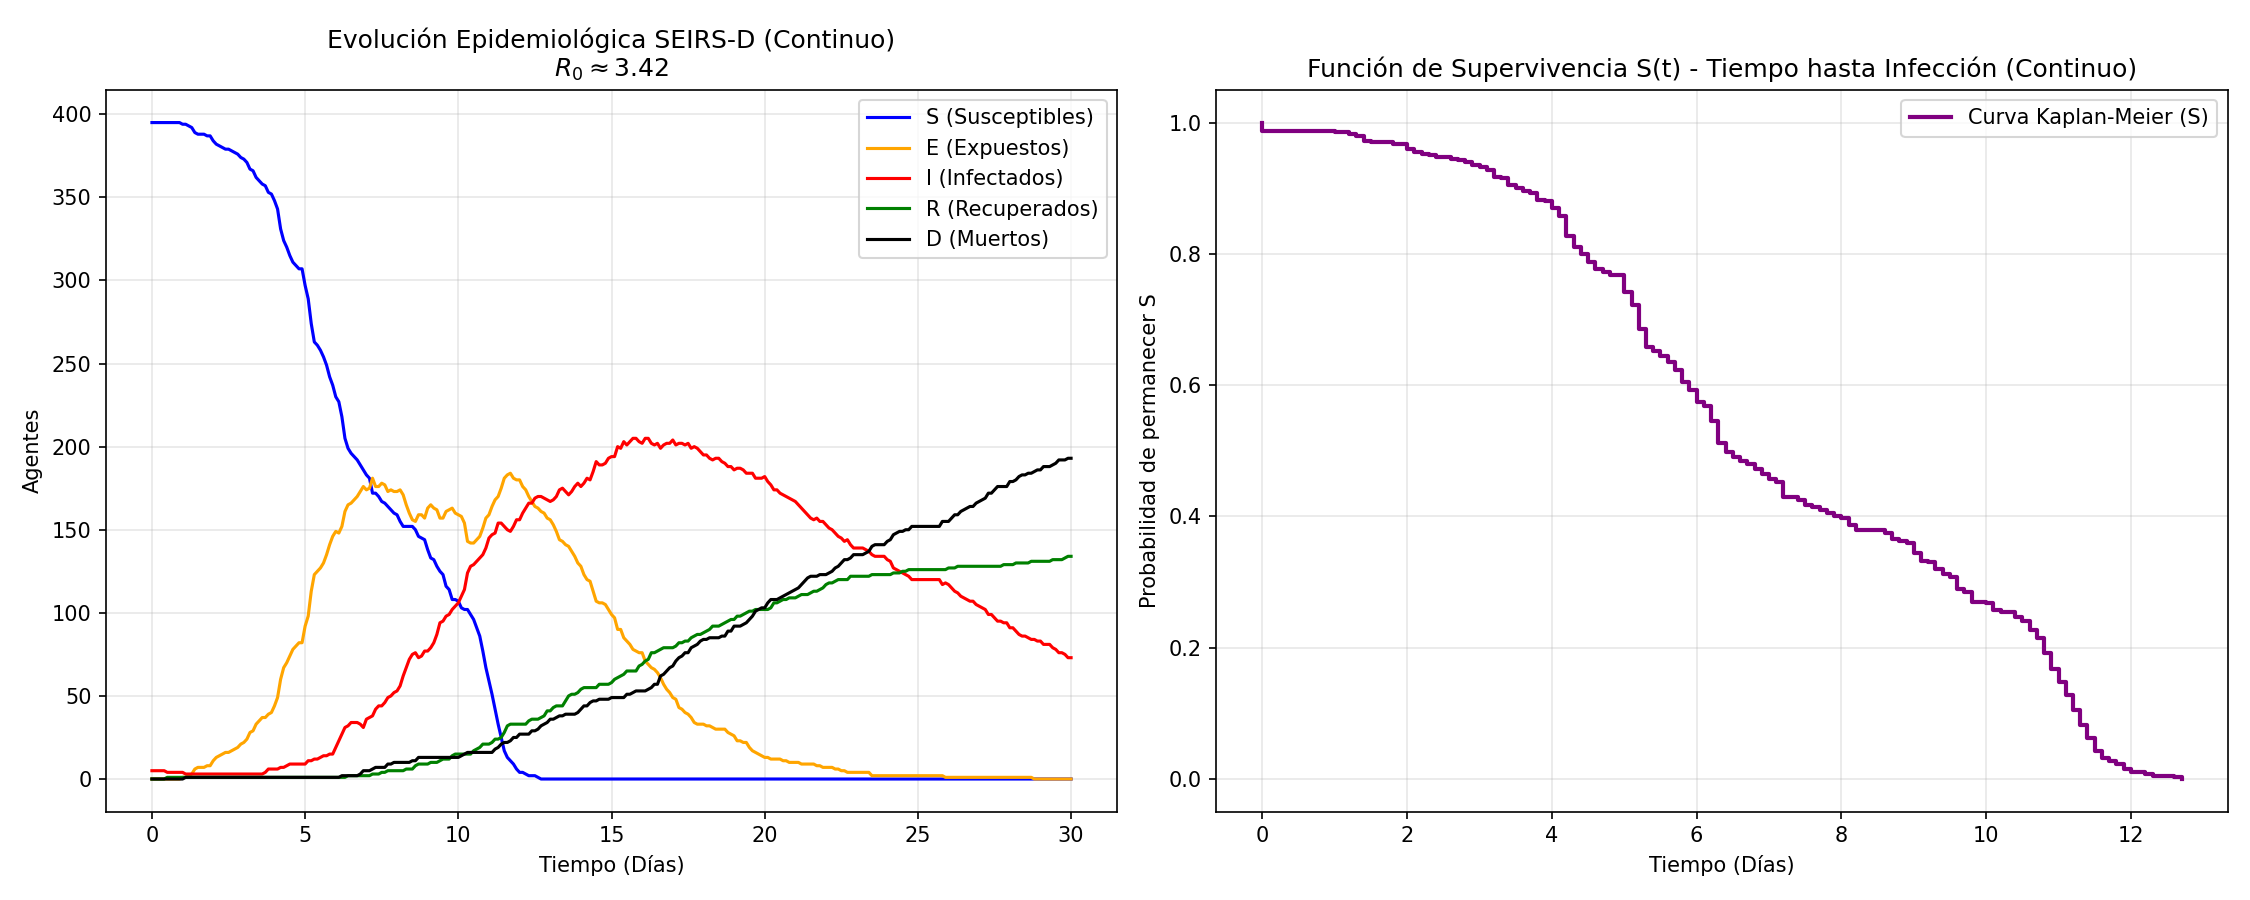
\includegraphics[width=0.45\textwidth]{analisis_continuo.png}
    \caption{Evolución temporal de los compartimentos y curva de supervivencia en el enfoque continuo.}
    \label{fig:analisis_continuo}
\end{figure}

\begin{figure}[!h]
    \centering
    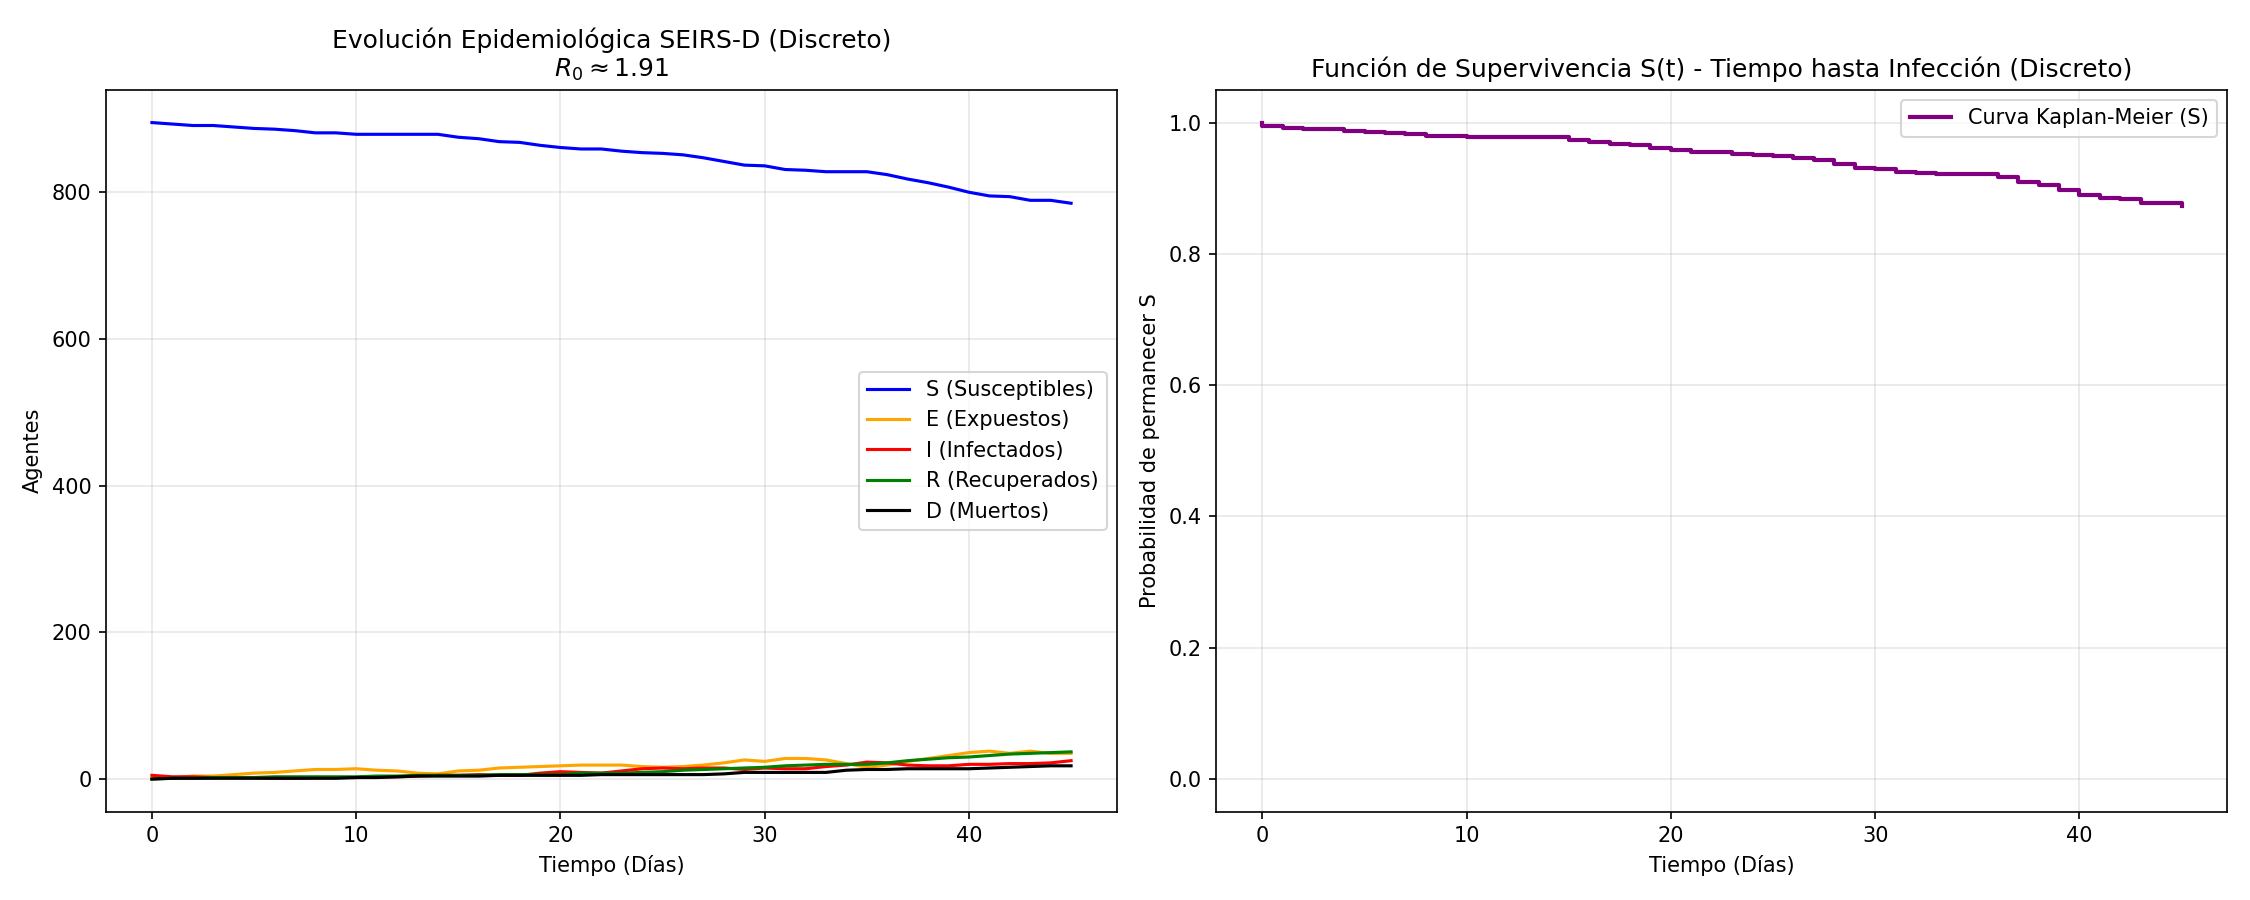
\includegraphics[width=0.45\textwidth]{analisis_discreto.png}
    \caption{Dinámica de propagación espacial y tasa de ataque en el enfoque discreto.}
    \label{fig:analisis_discreto}
\end{figure}

\subsection{Análisis de Sensibilidad Global de Sobol}
Para determinar qué componentes rigen la varianza de la tasa de mortalidad final, se ejecutó la descomposición global de Sobol mediante el estimador de Jansen ($N = 500$ muestras de Saltelli). El gráfico descompone los factores dividiendo las respuestas en dos dimensiones: el \textit{Efecto Directo} (barra cian: impacto del parámetro por sí solo, $S_i$) y el \textit{Efecto Total} (barra roja: impacto sumando sus interacciones no lineales con las demás variables, $S_{Ti}$), reportados en la Fig. \texttt{analisis\_sobol.png}.

\begin{figure}[!htbp]
    \centering
    
\includegraphics[width=0.48\textwidth]{analisis_sobol.png}
    \caption{Índices de sensibilidad global de Sobol calculados mediante el estimador robusto de Jansen ($N = 500$ muestras de Saltelli) para la varianza de la Tasa de Mortalidad.}
    \label{fig:analisis_sobol}
\end{figure}

El comportamiento de los índices permite estructurar el impacto en tres dimensiones analíticas:

\begin{enumerate}
    \item \textit{El Bloque Clínico domina el impacto directo:} La Pendiente de Letalidad ($\lambda$) y el Peso del Estrés por Viremia ($w_1$) presentan los efectos directos más masivos del sistema ($S_i = 0.94$ y $S_i = 0.88$, respectivamente). Esto demuestra que, una vez que el patógeno infecta a la población, el colapso biológico y el desenlace terminal de los agentes se deciden de forma casi lineal por estos dos parámetros internos del huésped.
    
    \item \textit{La Cópula ($\rho$) como pilar genético:} El coeficiente de acoplamiento inmunológico de la cópula ($\rho$) adquiere un rol protagónico con un índice directo robusto ($S_i \approx 0.42$). Este hallazgo demuestra cuantitativamente que el grado de deterioro sistémico correlacionado de la población explica por sí solo una fracción sustancial de la varianza de la mortalidad. Asimismo, su efecto total roza la unidad ($S_{Ti} \approx 1.00$), confirmando que interactúa de forma masiva con las variables dinámicas a lo largo de la simulación.
    
    \item \textit{Las Variables Ambientales como catalizadores no lineales:} Con excepción del Decaimiento Viral en Exteriores ($\delta_{ext}$), el cual opera como un límite lineal absoluto ($S_i = 1.00$), los parámetros físicos del Radio del Aerosol ($\ell$) y la Tolerancia Inmune de Dosis ($\tau_{max}$) presentan efectos directos moderados o bajos ($S_i \approx 0.32$ y $S_i \approx 0.07$), pero efectos totales sumamente elevados ($S_{Ti} \approx 0.96$ y $S_{Ti} \approx 0.72$). Esto confirma que las variables físicas del entorno no determinan la muerte de forma directa, sino que regulan cinemáticamente el volumen y la velocidad macroscópica del contagio, delegando la letalidad última a la resolución inmunológica interna del huésped.
\end{enumerate}


\section{Discusión}

\subsection{Explicación Física de los Hallazgos}
La gran diferencia entre los valores de $R_0$ obtenidos empíricamente y los de la literatura se explica por la estocasticidad espacial. En una población de tamaño acotado ($N = 400$), un paciente cero que inicie su rutina cerca de un \textit{hub} cerrado (como una escuela o lugar de trabajo) gatillará un brote superpropagador instantáneo debido al bajo decaimiento de aerosoles en interiores ($\delta_{cerrado} = 0.2$), arrojando estimaciones de $R_0$ superiores a $20$. 

En contraparte, si la infección inicial queda confinada en hogares periféricos aislados, el brote puede extinguirse rápidamente con un $R_0 < 3$. Esto confirma que el $R_0$ medido en modelos basados en agentes (ABM) espaciales es una propiedad emergente del comportamiento geográfico y no una constante fija del patógeno.

\subsection{Implicancia de las Intervenciones y Mascarillas}
Los resultados justifican el modelado de la mascarilla como un filtro asimétrico bidireccional:
\begin{itemize}
    \item La reducción de la emisión del exhalador infectado $(1 - \eta_{em})$ evita la saturación de aerosoles en las micro-zonas de los \textit{hubs}.
    \item La filtración del receptor susceptible $(1 - \eta_{rec})$ ralentiza la absorción acumulada de la dosis por debajo del umbral $\tau_{infection}$.
\end{itemize}

El acoplamiento no lineal de ambos factores (cumplimiento comunitario frente a eficiencia material) demuestra que las campañas orientadas a elevar el porcentaje de uso de barbijos son más efectivas para mitigar epidemias de aerosoles que simplemente mejorar la calidad técnica de mascarillas individuales en poblaciones de bajo cumplimiento.

\subsection{Limitaciones del Modelo}
\begin{itemize}
    \item \textit{Simplificación del Espacio:} El modelo asume un entorno continuo libre de obstáculos (paredes físicas) en los \textit{hubs}, reduciendo la física del aerosol a un \texttt{KDTree} isotrópico.
    \item \textit{Ausencia de Redes de Transporte:} El tránsito de los agentes se realiza mediante una interpolación rectilínea simple entre el hogar y el \textit{hub}, en lugar de modelar flujos vehiculares o peatonales complejos.
\end{itemize}

\section{Conclusión}
El marco SEIRS-D unifica la modelación epidemiológica clásica y estocástica basada en agentes. Al acoplar trayectorias virales individuales gobernadas por SDE-OU con un estado inmunológico correlacionado por cópulas, el simulador elimina la homogeneidad artificial de los modelos tradicionales y permite evaluar de manera intercambiable mecanismos de contagio por vecindad discreta o difusión continua de aerosoles, manteniendo una base biológica común inmutable.

\bibliographystyle{IEEEtran}
\begin{thebibliography}{1}
\bibitem{jansen}
A.~Jansen, ``Global sensitivity analysis: The tuning of random coefficient models,'' \emph{Particle Systems Analysis}, vol. 14, no. 2, pp. 112--124, 1999.
\end{thebibliography}

\end{document}